%%TITRE
\begin{center}
    \textbf{\Large ANALYTICS AUTOMATIZATION IN INDUSTRY} \\
    \vspace{0.5cm}

    Miniconference Report \\
    CHAU Dang Minh
\end{center}

\begin{center}
    \begin{minipage}{0.85\textwidth}
        \textbf{Summary.} Mr. Grégoire de Lassence, a data scientist at SAS, expounded the importance of Analytics Automatization in the industrial context, and gave a tutorial on SAS analytical tools.
    \end{minipage}
\end{center}

\section{The Problem}
As data becomes larger in volume and variety, and higher in velocity and veracity. Novel methods need to be adapted to analyze the data. These methods require collaboration among experts in IT (architectures, securities), Analytics (statisticians, data scientists, mathematicians) and Business (data analysts). When coming to automatization, a circle of development must be established. Analytics goes from cleaning the data, descriptive analysis, predictive analysis. The ultimate goal of analytics is to adjust actions for the best outcome in the future. Ontologically, the process goes through data, information, knowledge and intelligence.

\section{Tutorials}
The software provided by SAS implemented a user-friendly interface that allows interactive model building. This is the first step in analytical automatization comparing to hard code. The software can be considered as Power BI for data scientists as it is more flexible in model building. An illustration of using Decision tree is shown in Figure \ref{fig:sas}.

\begin{figure}[ht]
    \centering
    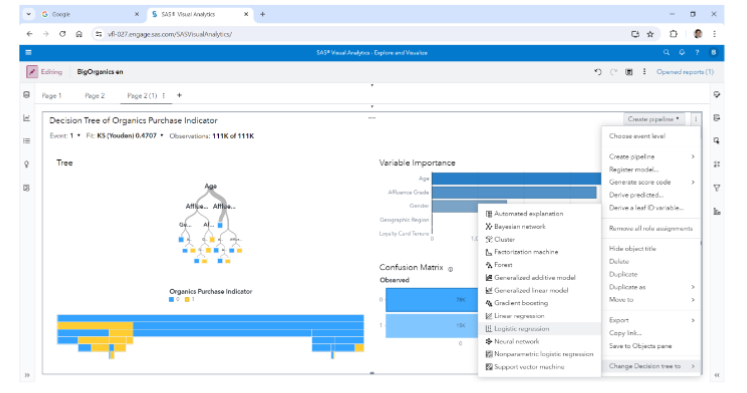
\includegraphics[width=\textwidth]{img/sas.png}
    \caption{SAS Analytical Interface for Modeling Building}
    \label{fig:sas}
\end{figure}

\section{Conclusion}
In conclusion, though learning to use a software does not require an in-class tutorial, it has been pointed out that automatization in analytics is necessary, especially for big data.

